% CREATED BY DAVID FRISK, 2016

% IMPORT SETTINGS
\documentclass[12pt,a4paper,twoside,openright]{report}
\input{Settings}

\begin{document} 

% COVER PAGE, TITLE PAGE AND IMPRINT PAGE
% Roman numbering (starting with i (one)) until first main chapter
\pagenumbering{roman}

%%%%%%%%%%%%%%%%%%%%%%%%%%%%%%%%%%%%%%%%%%%%%%%%%%%%%%%%%%
% NOTE(Bjorn):Global Variables for the frontmatter section.
%%%%%%%%%%%%%%%%%%%%%%%%%%%%%%%%%%%%%%%%%%%%%%%%%%%%%%%%%%
% An Informative Headline describing\\ the Content of the Report
\newcommand{\varHeadline}{Sphere Tracing GPU}
% A Subtitle that can be Very Much Longer if Necessary
\newcommand{\varSubtitle}{A Graphics Processing Unit Designed to Use Sphere 
	Tracing for Rendering}
% Department of Some Subject or Technology
\newcommand{\varDepartment}{Department of Computer Science and Engineering}
% Division of Division name
\newcommand{\varDivision}{Undergrad}
% Name of research group (if applicable)
\newcommand{\varResearchGroupName}{DATX02-17-12}
% NAME FAMILYNAME
\newcommand{\varNames}{
	Jesper Åberg\vspace{2mm}\\
	Björn Strömberg\vspace{2mm}\\
	André Perzon\vspace{2mm}\\
	Chi Thong Luong\vspace{2mm}\\
	Jon Johnsson\vspace{2mm}\\
	Elias Forsberg
}

\newcommand{\clash}{C$\lambda$aSH}

%zipwith
\makeatletter
% \zipwith{<coupler>}{<list1>}{<list2>}{<return macro>}
% \zipwith*{<coupler>}{<listcmd1>}{<listcmd2>}{<return macro>}
\protected\def\zipwith{%
  \begingroup
  \@ifstar{\def\cnta{1}\@zipwith}
    {\def\cnta{0}\@zipwith}%
}
\def\@zipwith#1#2#3#4{%
  \def\tempa##1##2{%
    \edef##2{%
      \ifnum\cnta=\@ne\else\expandafter\@firstoftwo\fi
      \unexpanded\expandafter{##1}%
    }%
  }%
  \tempa{#2}\tempb\tempa{#3}\tempa
  \def\cnta{0}\def#4{}%
  \foreach \x in \tempb{%
    \xdef\cnta{\the\numexpr\cnta+1}%
    \gdef\cntb{0}%
    \foreach \y in \tempa{%
      \xdef\cntb{\the\numexpr\cntb+1}%
      \ifnum\cntb=\cnta\relax
        \xdef#4{#4\ifx#4\empty\else,\fi\x#1\y}%
        \breakforeach
      \fi
    }%
  }%
  \endgroup
}
\makeatother

%scatter plot command
%usage: 
%  \scatterplot{x1,x2,x3...}{y1,y2,y3}{xscale}{yscale}{xlabel}{ylabel}{datafile}
%    where datafile is a file with a list of x y coordinates (one space 
%    separated pair on each line)
\newcommand{\scatterplot}[7]{
	\begin{tikzpicture}[only marks, y=.5cm]
		\draw[->,xshift=-5.0cm] (5.0,0) -- coordinate (x axis mid) (14,0);
		\draw[->,xshift=-5.0cm] (5.0,0) -- coordinate (y axis mid) (5.0,14);
		\zipwith{/}{0,1.6,3.2,4.8,6.4,8}{#1}\xlist
		\foreach \x/\xtext [evaluate=\x as \xeval using 2*\x] in \xlist
			\draw (\x cm,1pt) -- (\x cm,-6pt)
			node[anchor=north] {$\xtext$};
		\zipwith{/}{0,1.3,2.6,3.9,5.2,6.5}{#2}\ylist
		\foreach \y/\ytext in \ylist
			\draw (1pt,\y cm) -- (-3pt,\y cm) 
			node[anchor=east] {$\ytext$};
		\node[below=1cm] at (x axis mid) {#5};
		\node[anchor=south,left=1.5cm,rotate=90] at (y axis mid) {#6};
		
		\foreach \ys [evaluate=\ys as \ysc using 0.01*\ys] in {#4} {
			\foreach \xs [evaluate=\xs as \xsc using 0.1*\xs] in {#3} {	
				\draw plot[y=\ysc cm,x=\xsc cm,mark=*] file {#7};
			}
		}
	\end{tikzpicture}
}

% CREATED BY DAVID FRISK, 2016

% COVER PAGE
\begin{titlepage}
\newgeometry{top=3cm, bottom=3cm,
			left=2.25 cm, right=2.25cm}	% Temporarily change margins		
			
% Cover page background 
\AddToShipoutPicture*{\backgroundpic{-4}{56.7}{figure/auxiliary/frontpage_eng.pdf}}
\addtolength{\voffset}{2cm}

% Cover picture (replace with your own or delete)		
%\begin{figure}[H]
%\centering
%\vspace{2cm}	% Adjust vertical spacing here
%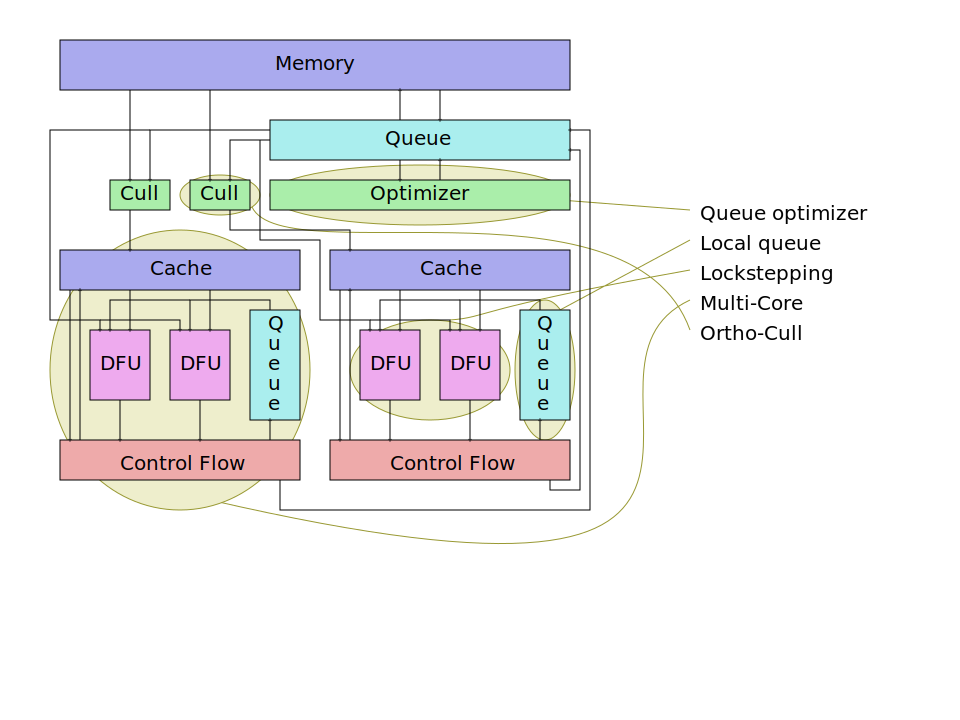
\includegraphics[width=0.9\linewidth]{figure/hardware_beta.pdf}
%\end{figure}

% Cover text
\mbox{}
\vfill
\renewcommand{\familydefault}{\sfdefault} \normalfont % Set cover page font
\textbf{{\Huge{}\varHeadline}} 	\\[0.5cm]
{\Large \varSubtitle}\\[0.5cm] Bachelor's thesis in Computer Science and Engineering \setlength{\parskip}{1cm}

{\Large \varNames} \setlength{\parskip}{2.9cm}

\varDepartment \\
\textsc{Chalmers University of Technology} \\
Gothenburg, Sweden, July 2017

\renewcommand{\familydefault}{\rmdefault} \normalfont % Reset standard font
\end{titlepage}

% TITLE PAGE
\newpage
\thispagestyle{empty}
\begin{center}
	\textsc{\large Bachelor of Science Thesis}\\[4cm]		% Report number given by department 
	\textbf{\Large \varHeadline} \\[1cm]
	{\large \varSubtitle}\\[1cm]
	{\large \varNames}
	
	\vfill	
	% Logotype on titlepage	
	%\begin{figure}[H]
	%\centering
	% Remove the following line to remove the titlepage logotype
	%\includegraphics[width=0.2\pdfpagewidth]{figure/auxiliary/logo_eng.pdf} \\	
	%\end{figure}	\vspace{5mm}	
	
	\varDepartment \\
	\textsc{Chalmers University of Technology} \\
	Gothenburg, Sweden, July 2017 \\
\end{center}


% IMPRINT PAGE (BACK OF TITLE PAGE)
\newpage
\thispagestyle{plain}
\vspace*{4.5cm}
\varHeadline \\
\varSubtitle \\
\varNames \setlength{\parskip}{1cm}

\copyright ~ \varNames, 2017. \setlength{\parskip}{1cm}

%%name and company or department.
Supervisor: Miquel Pericas, Computer Science and Engineering\\
Examiner: Arne Linde, Computer Science and Engineering \setlength{\parskip}{1cm}

Bachelor's Thesis 2017:NN\\	% Report number given by department 
\varDepartment \\
\varResearchGroupName\\
Chalmers University of Technology\\
SE-412 96 Gothenburg\\
Telephone +46 31 772 1000 \setlength{\parskip}{0.5cm}

\vfill
% Caption for cover page figure if used, possibly with reference to further information in the report
Cover: The GPU as it stands, with additions marked out. \setlength{\parskip}{0.5cm}

Gothenburg, Sweden 2017



% ABSTRACT
\newpage
% CREATED BY DAVID FRISK, 2016
\varHeadline\\
\varSubtitle\\
\varNames\\
\varDepartment\\
Chalmers University of Technology \setlength{\parskip}{0.5cm}

\thispagestyle{plain}			% Supress header 
\setlength{\parskip}{0pt plus 1.0pt}
\section*{Abstract}
The aim of this project is to develop the fundamental building blocks for a real-
time 3D graphics processing unit (GPU) that is optimized to run a rendering 
algorithm which is different to the Polygon-based rendering that is almost 
exclusively used in today's 3D graphics cards. During the early 90’s many types of 
rendering algorithms were developed and used, since they all ran in software on the 
main computer processor. Better performance (better graphics) was a key selling 
point among competing computer systems, the computer industry moved towards 
dedicated hardware based rendering systems. These systems were almost exclusively 
using polygon-based rendering. Today, 3D graphics cards have become more 
programmable but are still based on the old paradigm of polygon rendering. The last 
5 years have seen a small resurgence in the use of a sphere tracing rendering 
algorithm known as Ray- Marching. This has a whole new set of pros and cons when 
compared to the polygon renderers.  However, while the algorithm seems to have a lot 
of potential for future 3D graphics, that potential might be unreachable on current 
GPUs due to the underlying architecture being designed with other things in mind. 
This project will examine what could be achieved if graphics cards were optimized 
for ray-marching instead of drawing polygons.  

% KEYWORDS (MAXIMUM 10 WORDS)
\vfill
Keywords: lorem, ipsum, dolor, sit, amet, consectetur, adipisicing, elit, sed, do.

\newpage				% Create empty back of side
\thispagestyle{empty}
\mbox{}


% TABLE OF CONTENTS
\newpage
\tableofcontents

%% OTHER FRONTMATTER
%% List of figures (add to table of contents)
%\cleardoublepage
%\addcontentsline{toc}{chapter}{\listfigurename} 
%\listoffigures
%% List of tables (add to table of contents)
%\cleardoublepage
%\addcontentsline{toc}{chapter}{\listtablename}  
%\listoftables

% START OF MAIN DOCUMENT
%\cleardoublepage
\newpage
\setcounter{page}{1}
\pagenumbering{arabic}
\setlength{\parskip}{10pt}
\setlength{\parindent}{0pt}

% INTRODUCTION
\chapter{Introduction} 	
%	\section{Background} 
	During the early '90s many types of real time rendering algorithms were 
	developed and tested \cite{TODO}. This was possible because they ran in 
	software on the CPU, and could thus be easily altered and enhanced. 
	Photo realistic rendering could be done using a method called Ray Tracing, 
	but this was very slow\cite{TODO}. Improvements were made to this method and 
	one such sub-algorithm was called Sphere Tracing. It proved useful for Ray 
	Tracing 3D fractals\cite{TODO}, but it was still too slow to render any type 
	of geometry in real time\cite{TODO}. Better graphics rendering (fast real 
	time graphics) was a key selling point among competing computer systems, so 
	to improve rendering speed, the computer industry moved towards dedicated 
	hardware based 	graphics rendering\cite{TODO}. These systems were almost 
	exclusively using polygon-based rendering, unsuitable for most Ray Tracing 
	algorithms. Today, 	3D graphics cards have become more programmable and the 
	last 5 years have seen a small resurgence in the use of Sphere Tracing 
	rendering\cite{TODO}. Simple scenes can now be rendered using Sphere Tracing 
	in real time using state-of-the-art consumer 3D graphics cards. However the 
	full potential of the algorithm might still be unreachable on current GPUs 
	due to the underlying architecture being designed for polygon rendering to a 
	large extent\cite{TODO}. This project examines what could be achieved if 
	graphics cards were optimized and built specifically for Sphere Tracing 
	Graphics instead of today’s Polygon Graphics.		 
	
	\section{Project goals}
	
		The main goal for this project is to design and implement a basic GPU 
		architecture that is designed to efficiently execute the Sphere Tracing 
		algorithm. In striving towards efficiency, we examine Sphere Tracing in 
		order to find possible optimizations, both algorithmic and hardware 
		based.
		
	\section{Scope}

		Writing a GPU for the first time, even a smaller one, and doing it well is a large undertaking for a single bachelor project. The project is therefore instead done on a best-effort basis where we try to get at the novel parts of the design, while leaving out generally well researched systems such as cache and memory management. 


% PROBLEM DESCRIPTION
\chapter{Problem Description}

	The main problem is to identify the critical parts of the algorithm that
	prevents it from being a feasible alternative today, and to figure out a
	 hardware design that improves the performance of those parts. Following are the
	questions we worked to answer throughout the project.
	
	\begin{itemize}
		\item How does sphere tracing work?
		\item What language is best suited to describe the GPU?
		\item Are there ways we can improve the algorithm at a theoretical 
			level?
		\item How do we architect for parallelism and multiple cores?
		\item How do we handle cache in a smart way?
		\item What mathematical functions are best implemented in hardware vs 
			software?
	\end{itemize}


% STATE OF THE ART / LITERATURE
\chapter{State of the Art}

	\section{ Real Time Graphics Rendering on Current Hardware } 

		Sphere tracing is currently being used to visualize complex data such
		as fractals \cite{TODO}, but there is no modern consumers graphics
		cards designed to run it efficiently.  Today's top of the line consumer
		3D graphics cards are made for real time rendering of
		polygons\cite{TODO}. They achieve good performance by executing
		rasterization and pixel color calculation in parallel between pixels.
		To make this efficient they use what is known as lockstepping, which
		means a group of calculation units that are always operating on the
		same instruction, but with differing input data. This enables all of
		the cooperating cores to use only a single instruction memory and bus.
		This reduces the area usage of the design, making it possible to add
		more cores per chip and thus achieve greater performance. Rendering
		using polygon based methods can usually be queued for calculation in
		such a way that pixels within the same object, for example a sphere, in
		the scene can be grouped for computation. The disadvantage of
		lock-stepped cores only being able to work on the same instruction at a
		time is thus greatly reduced.
		
		Using this hardware for Sphere Tracing, as is currently being done,
		increases the overhead caused by this lock-stepped design significantly. 
		Order of pixel rendering in a polygon renderer is done by object and 
		then by constituent polygons. Pixels can not be grouped by what object 
		in the scene they belong to as easily in a Sphere Tracer, because 
		Sphere Tracers do not have polygons and pixel order is usually based on 
		the output image pixel order. Even if more grouping was introduced to a 
		Sphere Tracer, the pixels in these groups differ much more in their 
		instruction execution path, since the algorithm is more repetitive and 
		often varies greatly in number of steps until completion.
		
	\section{ Hobbyists and Academia }

		Despite this, computer art hobbyists are using Sphere Tracing to
		produce quite stunning real time visuals on consumer PC's. They
		showcase the possibilities of the algorithm by reducing scene
		complexity and instead rendering using techniques that are commonly
		found in non real time Ray Tracers. Examples of such are true
		reflections and refractions, spacial repetition, object morphing and 3D
		fractals\cite{InigoQuilez}.  Inspired by research papers such as John
		C. Hart's 1996 paper\cite{Hart1996}, their success encouraged hobbyist
		to do academic research of their own, which led to new papers being
		written. A good example of this is the 2014 paper "Enhanced Sphere
		Tracing"\cite{Korndorfer2014}.

	\section{ Industry }		

		% Kanske helt orelevant ?
		There are as of today no big commercial applications using Sphere
		Tracing that we know of, but Ray Tracing algorithms have long been in
		use in multiple computer graphics domains. For instance in film making
		\cite{TODO}, where a comparatively large amount of time to render a
		scene can be acceptable but the value of realism is higher than in real
		time graphics. An example of this would be the Ray Tracing engine
		RenderMan developed by Disney Pixar which is used for their movies
		\cite{TODO}.
	
	\section{ Hardware Design Methods } 
	
		The design of Integrated Circuits in the hardware industry has since
		the early '90s primarily been done in hardware description languages
		(HDL) \cite{Chen2012}, where one describes the operation of a chip in a
		style similar to regular imperative programming languages. This
		descriptive code can then be compiled into a list of components and
		connections that constitutes the blueprint for that specific circuit.
		The most prevalent of these languages are VHDL and Verilog\cite{TODO}.
		While being great help to designers, compared to more manual design,
		these languages can be quite cumbersome to work with. They are verbose
		and require a fair amount of boilerplate code. This makes it more
		difficult to understand, follow, and also write code that performs
		complex tasks, since it can be more difficult to see the greater
		patterns in interconnecting code\cite{TODO}.
		
		This has resulted in Functional HDLs (FHDL): ``Functional hardware
		description languages are a class of hardware description languages
		that emphasize on the ability to express higher level structural
		properties, such a parameterization and regularity. Due to such
		features as higher-order functions and polymorphism, parameterization
		in functional hardware description languages is more natural than the
		parameterization support found in the more traditional hardware
		description languages, like VHDL and Verilog'' \cite{Baaij2009}
		
		HDLs have been around since the late '70s \cite{Chen2012}, but in
		recent times they have become more mature\cite{TODO}. There are in
		particular two FHDLs, \emph{Lava} and \clash \cite{Baaij2009,
		Bjesse1998}, that are implemented in Haskell. This allows the same
		interactive type checking and high-level simulation of the program that
		normal Haskell programs enjoy. This means that instead of simulating
		the underlying circuit directly which is more time consuming, the
		design can be tested repeatedly at a faster pace, allowing faster
		development. This high level simulation can also be done in an
		interpreter enabling easy and rapid testing of code. These are called
		read-eval-print-loop interpreters.


% THEORY
% CREATED BY DAVID FRISK, 2016
\chapter{Sphere Tracing} \label{spheretracing}

	The graphics rendering algorithm the GPU was designed for is called
	Sphere Tracing\cite{Hart1996}. The name comes from the technique where it
	uses spheres to incrementally advance a ray in 3D space. The method of
	advancing rays in general is called Ray Marching which in turn is a subset of
	Ray Tracing\cite{Whitted1980a}. Ray Tracing, then, is a way of wholly or
	partially render the world off of rays, cast from the eye of the observer
	into the scene. Sphere Tracing has been around since at least as early as the
	late eighties\cite{Hart1989} and Ray Tracing as early as the
	sixties\cite{Appel1968}.

	In this chapter the Sphere Tracing algorithm is lifted in detail with
	both definitions and examples. The explanation is based on the the very
	succinct explanation in \cite{Korndorfer2014}. The paper also expands upon
	the original algorithm in some innovative ways. For a more in-depth
	description of the original algorithm see Harts ``\emph{Sphere Tracing: a
	geometric method for the anti-aliased ray tracing of implicit
	surfaces}``\cite{Hart1996}.

	\section{Sphere Tracing} 

		\begin{wrapfigure}{r}{0.48\textwidth}
			\begin{flushright}
				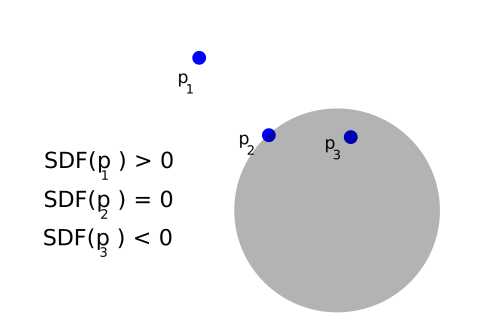
\includegraphics[width=0.9\linewidth]{figure/SDF} 
			\end{flushright}
			\caption{ Signed Distance Function of a sphere, sampled at three points}
			\vspace{40pt}Sphere Tracing
		\end{wrapfigure}

		The Sphere Tracing algorithm uses Signed Distance Functions (SDF).
		$$\text{SDF}:\mathbb{R}^{3}\mapsto\mathbb{R}$$ The ``distance`` is the euclidean distance between a point and the closest point on the implicit surface
		$\text{SDF}^{-1}(0)$. ``signed`` refers to the distance being
		negative when measured on the inside of an object. 

		A common example would be the SDF of a sphere centered at the origin with a
		radius of one. $$\text{SDF}(\vec{v}) = |\vec{v}| - 1$$ We can here see that
		a point $\vec{v}$ exactly on the surface would evaluate to $1 - 1 = 0$
		where any point outside of the sphere is positive and any point inside the
		sphere is negative. In this case the absolute value of the result would also
		describe the smallest distance to the surface but as long as the result is
		the smallest distance \emph{or greater}, the algorithm will work.

		If we define a ray $r$ $$r(s) = \vec{d} \cdot s + \vec{o}$$
		where $\vec{d}$ is the direction of the ray and $\vec{o}$ the origin, then
		$$\text{SDF}\circ r(s) = 0$$ means that the ray intersects a surface at
		exactly distance $s$ from the view point origin. Sampling every SDF in a
		given scene and returning the smallest value yields a function known as a
		distance field.

		\bigskip \noindent Finding the surface can be done by marching point by
		point from the origin along the ray like below: 
		
		$$p_{i+1} = p_i + \vec{d}\cdot \text{SDF}(p_i)$$ 
		
		\vspace{40pt}
		\begin{wrapfigure}{r}{0.48\textwidth}
			\begin{flushright}
				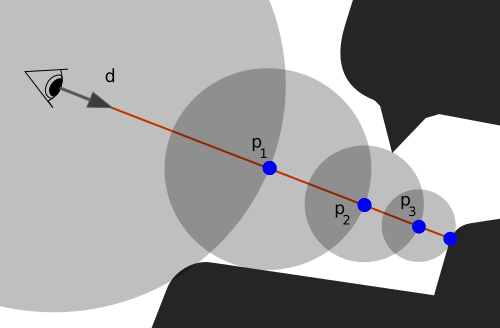
\includegraphics[width=0.9\linewidth]{figure/SDF2} 
			\end{flushright}
			\caption{A single ray marching according to Sphere Tracing}
			\vspace{40pt}
		\end{wrapfigure}

		This is repeated until $\text{SDF}(p_i) \leq \varepsilon$ for a given
		precision limit $\varepsilon$. $\text{SDF}(p_i)$ is the furthest possible
	 distance the ray can march while still not overshooting any potential
		surfaces. The direction to the closest surface point is never known, thus
		$\text{SDF}(p_i)$ can be interpreted as a spherical bound, giving the
		algorithm it's name. The Sphere Trace is performed for each pixel of the
		screen, reversely simulating the light rays entering the lens of an eye or
		camera.

			\subsection{Reflections, refractions and shading}

				Once a point on a surface for a given pixel has been located
				reflections, light, shadows and refractions can be calculated. These sometimes depend on the surface normal which can be approximated with
				the partial derivatives around the surface point given some small delta
				$\delta$. This is the normalized gradient $\vec{g}$ in this point.

				$$\vec{g} = \vec{x}\cdot\frac{\text{SDF}(x+\delta, y, z)}{\delta} +
				\vec{y}\cdot\frac{\text{SDF}(x, y+\delta, z)}{\delta} +
				\vec{z}\cdot\frac{\text{SDF}(x, y, z+\delta)}{\delta} $$

				$$\vec{n} = \frac{\vec{g}}{|\vec{g}|} $$

				A simple way to illuminate the scene could for an example be to use
				Phong Lightning\cite{Phong1975}. But any number of alternative
				algorithms could be used instead to determine the final color. Shadows
				can be determined by doing a new Sphere Trace, towards the sources of
				light to check for obstructions. Same for reflections and refractions
				where further marching in proportionate angles to the angle of
				incidence can determine what objects reflects on the surface.


% METHODS
\chapter{Implementation}

	In order to achieve the goals set in this project, two separate pieces of
	software and one piece of hardware were written. The software programs are
	two different implementations of a reference shader. The first of these was
	written in GLSL for traditional graphics hardware (in our case it was tested
	on a GeForce GTX 1060M), and the second is written in an assembly language
	we designed for the Sphere Tracing processor.
	
	It is here worth noting that a shader is an historical term that today in
	modern industry terms refer to the code running on the GPU as opposed to on
	the CPU. It is called a \emph{shader} because initially only the color and
	illumination where programmable where as today the GPUs become more
	generally programmable by the generation. Both of these shaders are
	described in section \ref{implshader}.
	
	The hardware is comprised of a multi-core programmable parallel processing
	unit designed for the Sphere Tracing algorithm, detailed in section
	\ref{implproc}. In addition to these, a simple software assembler was
	written for the assembly language used for the GPU.
	
	Before any actual sphere tracing is done some essential values are
	calculated from predefined parameters. To have a functional sphere tracer a
	camera point and direction to look needs to be defined, in practice this is
	done by having an eye-vector and a vector that describes the point that the
	camera should be oriented against. From these vectors a new direction vector
	is calculated that defines the direction that the camera is oriented. The
	camera-vector is used as a origin for rays and the direction-vector is used
	to calculate the direction of each ray.
	
	The core of the Sphere Tracer is a simple while-loop. It begins by
	calculating the distance to the closest object in the scene by sampling the
	distance field and comparing its value at the current location to a
	predefined epsilon. If the value of the distance field is smaller than
	epsilon, the ray has hit an object. If no object has been hit, the sampled
	distance will be added to the length of the ray.

	\section{Reference Shader} \label{implshader}


		\subsection{GLSL Based}
	
			The shader is made to run on conventional graphics hardware, it was
			created in the high-level shading language GLSL (short for OpenGL
			Shading Language). It runs the program for each pixel the shader is
			rendered on, using the screen-coordinates as input.
			
			Before the loop is run Orthogonal Culling is executed, reducing the
			number of objects in the distance field. Beyond this, objects can
			also be enclosed in Bounding Spheres.
			
			After a hit is detected several different things will be done,
			depending on the material assigned to the object. If the object is
			reflective the normal of the surface hit is calculated and used to
			reflect the ray. If the object is colored the pixel will simply be
			set according to the object. Color can also be calculated from
			object or ray coordinates, coloring the pixel depending on where the
			object is or where it was hit.

		\subsection{Orthogonal culling}

			A bottleneck of Sphere Tracing is that the distance to
			a lot of objects has to be calculated once for every march step.
			One way to increase the performance is to reduce
			the number of objects that the distance has to be calculated to,
			without reducing the actual number of objects in the scene. To do
			this the GPU needs to calculate which object a ray might hit,
			traditionally the CPU will tell the GPU which objects are in the
			field of view (Frustum culling) but we can't do that because of
			GLSL does not allow us to run code on the CPU. Even if we could use frustum culling it would probably not be enough, each ray should only care for the objects that it might hit, not all objects in the field of view.

			Orthogonal projection works by going through all the objects in the 
			scene for ray and calculating if the ray can hit the object. 

			Orthogonal projection is used to tell whether a object is in front
			of the ray or not. By projecting the center of the sphere onto
			the directional line of the ray, its closest point to the line is
			known.  Then the distance between the line and the sphere can be
			calculated using the radius, if the distance is less than zero the
			sphere will be hit by the ray. If the distance is larger than zero
			the ray can't possibly hit that sphere. This way the number of
			objects that the distance has to be calculated to is decreased.

		\subsection{Bounding Spheres}
			
			To decrease the number of distance calculations that has to be
			performed in each march step is to enclose several objects in a
			Bounding Sphere. When the distance field is evaluated only the
			bounding sphere will be considered and none of the objects enclosed
			by it. If the bounding sphere is hit by the ray, it will be removed
			and all the contained objects will be introduced to the distance
			field.
			
			A Bounding Sphere is defined by it's location, radius and enclosed
			objects. The location is calculated by adding the position-vectors
			of objects and scaling the result with the inverse of the number of
			objects. The radius is the distance to the object that is the
			furthest from the Bounding Sphere's position added to that objects
			sphere of influence (how far it reaches from it's location). This
			way there is no risk of objects being partially rendered.


		\subsection{Assembler Based}

			In the assembler version that runs on our own hardware there is
			initially a single thread. This thread will create one new thread
			for each pixel on the screen, and this thread will calculate what 
			color the pixel should have and then terminate. This differs from 
			the shader version that simply runs the GLSL-code for each pixel
			in parallel at the graphics cards many cores.

	\section{Processor Unit} \label{implproc}

		The properties of the ray marching algorithm as described in chapter
		\ref{spheretracing} led to the decision of designing a GPU architecture
		that does not utilize multi-ALU SIMD with lockstepping to the same
		extent as that of traditional graphics processors. Instead, a solution 
		with slightly simpler independent cores was decided upon. This is 
		similar to reasoning employed by \cite{Woop2005} for a Ray Tracing 
		hardware design.

		The hardware described in this section was written in \clash. \clash is
		based on the functional programming language Haskell and is therefore a
		functional hardware description language, or FHDL. One thing that
		\clash offered was the command-line repl that allowed us to quickly
		write and test new modules on a higher conceptual level rather than
		simulating the Verilog code on a bit level.

		\subsection{Architecture}

			The GPU is designed to be able to handle a form of threading
			natively, where all computations are performed by a thread running
			on a hardware core. A thread in this context is very
			light-weight: only an instruction pointer along with some mutable
			registers are stored.

			All threads that are not running are sent to a storage manager that
			communicates with all cores, and threads are then dispatched to
			cores as the cores become available for execution.  The cores are
			also able to spawn new threads by sending their data to the storage
			manager, or terminate their current threads either by simply
			dropping them or by sending them to the frame buffer, where some of
			the registers will be used to determine the color of some pixel on
			the screen.

			Each core consists of instruction and data memories, some control 
			logic for execution order and a DFU. The data and instruction 
			memories are immutable and mirrored across all cores in their 
			entirety. The control logic is responsible for feeding the DFU with
			instructions and data, as well as updating the thread registers 
			when a new thread is attached, sending thread registers to the 
			storage manager when new threads are spawned and and 
			requesting a new thread whenever the previously executing one 
			terminates.
			
			The DFU contains a stack which all arithmetic instructions operate
			on, as well as an ALU for carrying out calculations. It also keeps
			track of all the thread registers and updates them when such
			instructions are issued. The DFU contains very little extra control
			logic and is only able to receive and execute instructions, it does
			not keep track of any instruction pointers or when threads are
			attached or dropped, this is instead handled by the core control
			logic.

		\subsection{Instruction Set}

			A representation for distance functions was also designed. It is
			implemented as a reverse polish notation inspired stack based 
			instruction set.

			There are a total of four instruction types with different
			instruction encodings, their layout in memory is shown in figure
			\ref{encodingfig}, and the type of instructions are:

			\begin{description}
				\item[C-type] instructions are for control flow, that is, 
					instructions that affect the global queue or frame buffer or
					terminate the current thread. C-type instructions can be 
					conditionally executed, based on the condition encoded in
					the two highest bits in the opcode. 

				\item[D-type] instructions, which encode arithmetic- and vector
					instructions on the stack. These operate only on the
					internal stack in the core and not on any of the other
					registers. They can take up to six arguments and return up
					to three return values. D-type instructions can be split up
					in chunks using the \texttt{next} instruction, where the
					last computed result will be accumulated using the minimum
					automatically by the core.  This is useful for encoding
					distance functions.

				\item[V-type] instructions deal with memory accesses. The
					\texttt{p} bit encodes whether this access is for pack
					(mutable) or read-only memory.

				\item[R-type] instructions load wide immediate values into the
					DFU. They are currently only used for assigning distance
					function IDs.
			\end{description}

		\subsection{Execution Model}

			The processor contains a global storage structure that is shared
			among all cores by a storage manager. All threads that are 
			ready for execution are held in this storage until a core is ready 
			to start executing them.

			\begin{figure}[H]
				\centering
				\caption{ XQBGPPPU Data flow diagram }
				\includegraphics[width=0.75\linewidth]{figure/dots/GPU-schematic} 
				\vspace{-4pt}
			\end{figure}
	
			Each shader thread has 16 mutable registers that are automatically
			loaded into the core when execution starts. These registers are
			saved when execution pauses and copied whenever a thread spawns a 
			new child. The instruction \texttt{setval} can be used to change 
			the value of a register, and the instruction \texttt{pack} reads 
			the value of a register.

			All calculations are performed with intermediate values stored on a
			stack, with the ability to move any values between the stack and
			any of the registers using the \texttt{setval} and \texttt{pack}
			instructions.

			There are three main instructions for control flow: \texttt{pushq},
			\texttt{pushf}, and \texttt{drop}. Threads can spawn new threads at
			any time using the instruction \texttt{pushq}: this will cause the
			core to make a copy of all of the registers and push it onto the
			global queue, where another (or the same) core may later access
			them and start executing from the instruction pointer register
			(\texttt{r0}).

			Threads can also terminate execution in two ways. Executing the
			instruction \texttt{drop} will terminate the thread and discard all
			registers. Executing \texttt{pushf} will terminate the thread and
			discard all values except the pixel pointer (\texttt{r1}) and color
			register (\texttt{r2}), which will be sent to the frame buffer in
			order to be displayed on the screen.

			This set of instructions for control flow might initially seem to
			be neither useful nor easy to implement but they are powerful
			enough to implement for all branching that is needed in our ray
			marchers efficiently while being restrictive enough to make
			instruction memory accesses very predictable.

			In addition to this, each core can accelerate finding the minimum 
			distance for a set of distance functions using a built-in 
			accumulator, together with the instructions \texttt{next} and 
			\texttt{accum}. Because of this, distance functions can be written
			without any regard for how the shader that called them works, and
			this very common operation is automated, reducing the size of each
			distance function slightly.

		\subsection{Square Roots}

			Calculating distances is an integral part of the algorithm, so a
			good square root implementation was considered important for
			achieving good performance. Several different approaches for this
			were considered.

			Firstly, using an iterative method like Goldschmidt's or the
			babylonian method was considered. These require an initial starting
			value, which is usually generated using a look-up table. We tested
			a different and very fast method for generating an initial rough
			guess of the square root of any number without the need for a
			look-up table. A 16-bit version of this circuit is shown in figure
			\ref{orsqrt}, and an improved but slightly more expensive version
			is showed in figure \ref{orsqrt2}.  The basic working principle is
			based on the fact that the square root of a number has roughly half
			as many digits as the original number. In the version with slightly
			improved accuracy the placement of the extra wires is based on the
			bit pattern of $\sqrt{2}$.

			\begin{figure}
				\centering
				\caption{A simple square root approximator}
				\label{orsqrt}
				\includegraphics[width=0.75\linewidth]{figure/pdf/simpleOr.pdf} 
			\end{figure}

			\begin{figure}
				\centering
				\caption{Simple square root approximator with minor improvement.
					This version includes an extra layer of or-gates with a
					shift of 4. Note that the gates in this diagram seem
					to be ordered in two extra layers. This is, however, only a
					visual artifact in this image. Adding more layers with
					shifts of 6, 10, 14, 26 etc increases accuracy further,
					although returns are diminishing quickly.}
				\label{orsqrt2}
				\includegraphics[width=0.75\linewidth]{figure/pdf/sqrt2Or.pdf} 
			\end{figure}

			In order to improve upon this method, both in terms of accuracy and
			stability, another design was considered in which the input was
			both rounded up and down to values where the simple square root
			approximator was very accurate and the result was then linearly
			interpolated between these roots. This linear interpolation
			requires only a multiplication and a couple of additions, but
			choosing upper and lower seed values is a more complex problem.
			Choosing the two geometrically closest powers of two was tested
			because the or-gate square root circuit is very accurate for powers
			of two, but this is not the only possible choice, as there are many 
			points for which the simple square root approximator is very 
			accurate. We did not look further into choosing different upper and
			lower bounds for the lerp-approximator.

			\begin{table}
				\centering
				\caption{A \texttt{C} implementation of the shifting nth root 
					algorithm}
				\label{sqrtc}
				\begin{tabular}{c}
				\begin{lstlisting}
int isqrt(int num) {
    int res = 0;
    int bit = 1 << 30;

    while(bit != 0) {
        if(num >= res + bit) {
            num -= res + bit;
            res = (res >> 1) + bit;
        } else res >>= 1;
        bit >>= 2;
    }
    return res;
}
				\end{lstlisting}
				\end{tabular}
			\end{table}

			\begin{table}
				\centering
				\caption{A \texttt{C} implementation of the shifting nth root
					algorithm. This code example is slightly longer, but
					relatively expensive additions have been replaced by
					bitwise ors.}
				\label{sqrtcopt}
				\begin{tabular}{c}
				\begin{lstlisting}
int isqrt(int num) {
    int res = 0;
    int bit = 1 << 30;

    while(bit != 0) {
    	int tmp = num - (res | bit);
    	res >>= 1;
        if(tmp >= 0) {
            num = tmp;
            res |= bit;
        }
        bit >>= 2;
    }
    return res;
}
				\end{lstlisting}
				\end{tabular}
			\end{table}

			Another algorithm for calculating square roots is the
			\emph{Shifting nth root algorithm}, also known as \emph{Dijkstras
			square root algorithm}, which calculates the square root one digit
			at a time. A \texttt{c} implementation of this algorithm is shown
			in figure \ref{sqrtc}. Initially, this algorithm does not seem like
			a good canditate for a high performance hardware implementation,
			but several important optimizations are possible when unrolling it
			combinatorially. Most of the additions can be reduced to bitwise
			logic operations already when computing it in software, as shown in
			figure \ref{sqrtcopt}. In a combinatorial hardware implementation,
			these bitwise operations can be removed entirely by simply moving
			wires around, yeilding a logic cost of 0. The only remaining
			operations is therefore the subtraction on line 6, and the
			conditional assignments of \texttt{num} and \texttt{res} on lines 9
			and 10. The cost of the subtraction can be significantly reduced
			because \texttt{res} approximates the result one bit every step,
			meaning most bits of \texttt{num} and \texttt{res} are zeroed at
			any given iteration. This means that on average, only 25\% of the
			subtraction logic is needed. This turned out to result in a design
			very similar to the PARSQRT implementation by \cite{Li}.


% RESULTS
\chapter{Results}

	In this chapter the results of GPU design choices and algorithmic
	optimizations and their effects are reviewed.

	\section{Software Shader Performance}

		The shader performed as expected, a conventional graphics card is 
		capable of rendering scenes with low scene complexity in real-time
		using sphere tracing.

		However scenes can easily be made to look a lot more complex than they
		are, for example, by using mod fields,or modulo fields, when the modulo
		operation is used on an object it creates a field with multiple copies
		of the original object next to each other, or fractals. The hardware
		(Geforce GTX 1060M) that the shader was tested on was able to render 20
		reflective spheres in real time in fullHD using our performance
		enhancing algorithm.


	\section{GPU}
	
	The GPU has been tested by simulating it and running a program on it that 
	renders a sphere using Sphere Tracing. It spawns threads progressively to 
	fill the screen data buffer with pixels. The execution of our test programs 
	ran exactly as intended, with any number of simulated cores. The design has 
	also been put through a synthesizing tool for FPGAs, which creates a net 
	list of the components and connections that constitute the GPU. This also 
	works as intended without any unexpected problems, but the actual operation 
	of the GPU on an FPGA has not yet been verified.
	
	
	\section{Square roots}
		
		The accuracy of the different square root approximation and calculation
		methods are shown in figures \ref{sres1}, \ref{sres2}, \ref{sres3},
		\ref{sres4}, \ref{sres5}, and \ref{sres6}. The shifting nth root
		algorithm is used as a reference in all figures because it is always
		bit-accurate for integer square roots.

		\begin{figure}[H]
			\centering
			\includegraphics[width=0.75\linewidth]{figure/value12x.png} 
			\caption{Value from the simple square root approximator (green),
				the improved version (blue), and the shifting nth root 
				algorithm (red).}
			\label{sres1}
		\end{figure}

		\begin{figure}[H]
			\centering
			\includegraphics[width=0.75\linewidth]{figure/rel_error_480x.png} 
			\caption{Relative error for the simple square root approximator
				(green), the improved version (blue), and the shifting nth root
				algorithm (red).}
			\label{sres2}
		\end{figure}

		\begin{figure}[H]
			\centering
			\includegraphics[width=0.75\linewidth]{figure/abs_error_24x.png} 
			\caption{Absolute error for the simple square root approximator
				(green), the improved version (blue), and the shifting nth root
				algorithm (red).}
			\label{sres3}
		\end{figure}

		\begin{figure}[H]
			\centering
			\includegraphics[width=0.75\linewidth]{figure/value_lin12x.png} 
			\caption{Value from lerp-approximator (purple), simple square root
				approximator with one step of the babylonian method (green),
				and the shifting nth root algorithm (red).}
			\label{sres4}
		\end{figure}

		\begin{figure}[H]
			\centering
			\includegraphics[width=0.75\linewidth]{figure/rel_lin960x.png} 
			\caption{Relative error for the lerp-approximator (purple), simple 
				square root approximator with one step of the babylonian method 
				(green), and the shifting nth root algorithm (red).}
			\label{sres5}
		\end{figure}

		\begin{figure}[H]
			\centering
			\includegraphics[width=0.75\linewidth]{figure/abs_lin24x.png} 
			\caption{Absolute error for the lerp-approximator (purple), simple 
				square root approximator with one step of the babylonian method 
				(green), and the shifting nth root algorithm (red).}
			\label{sres6}
		\end{figure}

	\section{Optimizations}
		
		During this project, a number of optimizations were discussed and
		developed. Implemented optimizations are explained below and the 
		theoretical ones are brought up in chapter \ref{discussion} and \ref{optimization}. 
		Some of these are based on earlier work, with some others believed 
		to be quite unique optimizations that have not been discussed for 
		sphere tracing previously. All implemented optimizations that affects
		the algorithm were implemented in the software shader, not on our own
		GPU.

		\subsection{Orthogonal culling}
		
		Tests to see the performance of the orthogonal culling optimization
		were performed by putting an increasing number of
		solid-colored spheres in a plane in front of the camera. Because of
		this, the spheres are not obstructed by other spheres, making this
		the best possible scenario for the optimization.

		Below are test results from Orthogonal culling.

			\begin{table}
			\centering
			\begin{tabular}{lll}
				\hline
				Objects & Optimized & Unoptimized \\ 
				\hline
				1       & 600       & 350         \\ 
				5       & 430       & 180         \\			
				10      & 290       & 98          \\
				15      & 85        & 13          \\
				20      & 58        & 9           \\
				25      & 40        & 6           \\
				30      & 29        & 4           \\
				35      & 7         & 3           \\
				40      & 6         & 2           \\
				45      & 4         & 1.5         \\
				\hline
			\end{tabular}
			\caption{Frames generated per second using the GLSL shader with and
				without the orthogonal culling optimization.}
			\end{table}

			%CHARTS
			
			\begin{table}
			\centering
			\scatterplot{1,2,10,15,20,25}{50,100,150,200,250,300}{4}{0.33}
				{frames}{number of objects}{/figure/OptimizedGraf.txt}
			\end{table}



%  \scatterplot{x1,x2,x3...}{y1,y2,y3}{xscale}{yscale}{xlabel}{ylabel}{datafile}
%    where datafile is a file with a list of x y coordinates (one space 
%    separated pair on each line)






			The tests were performed by putting an increasing number of
			solid-colored spheres in a plane in front of the camera. Because of
			this, the spheres are not obstructed by other spheres, making this
			the best possible scenario for the optimization.

		\subsection{Bounding spheres}

			Bounding spheres were implemented and tested. There was a clear
			gain in performance in some cases, but the results are very situational, 
			depending on too many factors to be able to review (number of objects, 
			the dispersion of objects, size and place of the bounding sphere, etc.). 
			The larger the bounding sphere, the less performance gain will be seen 
			and the more objects that can fit into a bounding sphere the more performance 
			gain will be seen. 


% DISCUSSION
\chapter{Discussion} 

	This chapter will discuss our thoughts on our result, our theoretical not 
	yet	implemented optimizations, and what future work is possible from this 
	point in time.
	
	\section{Results}  \label{discussion}
		
		\subsection{Software Shader}
		
            The optimizations that were implemented improved performance more than anticipated. There are many optimizations that are yet to be implemented and tested
            and it's hard to estimate the potential achievable performance, the
            only thing that is certain is that there are massive performance 
            potentials.

            There are great limitations in what could be done with the shader because of the language that we chose to implement it in, GLSL. It offers nothing more than a way to write a program which will run on a per-pixel basis and put the result on the screen. Because of this, CPU-GPU cooperation is not possible and that comes with consequences.

			Modern graphics engines not only does a lot of work on the CPU but it
			has granular control over the GPU, whereas we have no control at
			all. Things such as object positioning, frustum culling, etc.
			should be done by the CPU, not the GPU. This kind of implementation
			can not be done in GLSL and therefore a high-performance sphere
			tracer should be done not in GLSL but in a lower-level language.

            Although GLSL has it's limits it still has some very attractive 
            features, it was easy to learn because the syntax has much in common
            with java, which we've studied. The time it takes to develop new 
            features and test them is short. The purpose of the software shader 
            was to study the algorithm, implement and test optimizations and
            develop new features. For the purposes of this sphere tracer GLSL
            was a perfect fit.


		
		\subsection{GPU} 
		
			The project originally intended to create a simple single-core GPU
			that could fully render a scene given enough time, and then add on
			components as time allowed. Every design decision one makes clarifies what further needs to be done and reveals previously unseen flaws in the design that needs to be resolved. In the end we implemented the core and enabled multiple cores running in parallel utilizing a storage manager.  
			
            If we were to continue working ong on this project another workflow
            would be adopted when developing the GPU. More detailed planning is 
            required in the early stages and empiric testing of different 
            implementations is required along the entire development to reach
            the best possible solution.

	\section{Optimizations} \label{optimization}

		\subsection{Bounding spheres}
			
			Although an increase in performance could be seen using this
			method, it can also be used in ways that decreases the performance.
			By setting up a too large bounding sphere or my setting it up with
			few objects or simply objects that are far apart.

			To use this optimization efficiently the objects inside a bounding 
			sphere should never come far apart and the sphere should be exactly 
			the right size.

		\subsection{Orthogonal culling}

			The performance gain from this optimization exceeded our 
			expectations. This could probably be further improved by using
			another way to create the sphere tracer than GLSL. 

			However great the performance gain the way this is implemented
			is still far from the optimal solution, currently it performs orthogonal culling on all the objects in the scene per pixel. Instead,
            culling should be done on a per-object basis and calculate
            which rays an object intersects, this way fewer calculations would
            have to be performed and optimally they would be performed on the

			CPU.

			This method could work together with the Bounding Sphere 
			optimization. Instead of projecting single objects onto the ray,
			bounding spheres could be culled, decreasing the number of 
			orthogonal projections that has to be made. This too was tested 
			and an increase in performance was observed.

	\section{Square roots}

		The simple square root approximator and its improved version are
		extremely simple circuits, indeed they are signifcantly smaller than
		most other common operations performed on numbers in hardware. Of
		course, they are far from accurate, but we find it interesting that it
		is possible to acheive a bounded relative error from the true square
		root for any number of input bits with these small circuits. When
		combined with linear interpolation or iterative methods like the
		Babylonian method the accuracy of these approximations increases 
		signifcantly.
		
		The shifting nth root algorithm is the only bit-accurate method tested,
		and it performs well, albeit slower than the approximations. If
		non-exact results are acceptable, which they often are to some extent
		when doing sphere tracing, the number of steps in the shifting nth root
		algorithm could be reduced, which would both increase speed and
		decrease area usage. The lerp-based and iterative methods might still
		be able to reuse common components such as adders and multipliers 
		however, and might therefore be preferable.
		
		For the XQBGPPPU, we have used the shifting nth root algorithm in order
		to not have to consider possible accuracy problems when debugging 
		shaders, but all methods are implemented and ready to be switched out
		at any time.

	\section{Future work}

		\subsection{GPU-CPU cooperation}

            In the current implementation everything is performed on the GPU,
            including object transformations and culling. Currently if objects 
            in the scene are supposed to move they have to be moved using 
            mathematical functions, such as sinus. These functions are then evaluated for each march step. This is essentially wasted computing power and could be performed on the CPU as is standard in modern graphics engines.



		\subsection{Plane-ray intersection}

			Infinite planes currently require a lot of computing power to
			render. When the camera is oriented so that the field of view is
			along an infinite plane some rays will travel parallel to the
			plane. These rays will march equally long steps until their max
			number of steps has been taken or the max range has been reached, without hitting anything. This will cause some rays to draw computing power without ever being able to hit the plane anyway. Some rays that should hit the plane will fail to do so because of to many steps taken, making it look like the plane has an edge because after a certain range it is no longer being rendered.


			One potential problem is that because no distance field evaluations 
			are performed, it might be hard to perform Boolean operations or 
			mathematical deformations on planes rendered this way. Another is 
			that every time we add more features that aren't part of the regular 
			Sphere Tracing, the complexity of the program increases. Thus, the 
			advantages of the individual optimizations must be weighed against 
			the overall performance loss they incur. 

		\subsection{Overstepping}

			Bounding spheres technique is somewhat similar to the normal sphere
			tracing. The difference is that when you march you march to the
			edge of the MDS and then you march to the next MDS edge. With
			overstepping technique you march a small distance further
			outside the MDS edge. You then compare the original MDS with the
			new MDS if these two spheres overlap in any way we can march that
			little bit further. By marching that little bit further, decrease
			in the number of times marched is achieved. Giving an increase in
			performance. 

			%add link to mendeley paper
			
		\subsection{Ray grouping}
		
			Ray grouping works by grouping adjacent rays together.  If a specific
			pixel N is to be rendered we group the adjacent pixels into a set, then
			march along the ray of N. If any of the pixels are not inside the minimum
			distance spheres (MDS) the combined pixel is split up into smaller sets,
			which each have a centered pixel. Each set then repeats the these steps
			over and over again individually along their new center pixel's ray.
			This is repeated a number of times depending on the march distance in the
			scene for every set. The closer the sets are to a target, the more likely
			it is for a higher amount of subsets to be created due to the decrease of
			the MDS's volumes making less pixels fit inside.
			
			We believe ray grouping gives a performance increase by lowering the
			number of steps needed to march. Depending on the scene it could lower
			the steps significantly. One example would be a scene with only one
			object in it let's say a sphere, this implies that the MDS's volume will
			be substantial. This will in turn make the number of subgroups very low
			and give us a a performance gain. 
			
			A very complex scene with many objects creates very varying MDS volumes
			which would not give as good of a result as the earlier mentioned example
			due to the increase in subsets early in the marching.
			


% CONCLUSION
% CREATED BY DAVID FRISK, 2016
\chapter{Conclusion}
	\section{How does sphere tracing work?}

	\section{What language is best suited to describe the GPU?}
	
	The two FHDLs, lava2000 and \clash, not being fully developed languages both produced obtuse and redundant code and in the case of \clash even unsynthezisable code (bug). In the end we decided to go with \clash and it did allow us to type less and to have a more clear overview of the GPU and its components.

	\section{Are there ways we can improve the algorithm at a theoretical level?}



	\section{How do we architect for parallelism and multiple cores?}

	\section{How do we handle cache in a smart way?}

	\section{What mathematical functions are best implemented in hardware vs software regarding?}

% REFERENCES / BIBLIOGRAPHY
\cleardoublepage
\addcontentsline{toc}{chapter}{Bibliography}
% CREATED BY DAVID FRISK, 2016

\nocite{*}
\bibliographystyle{abbrv}
\bibliography{include/bibtex/DATX02-17-12}


% APPENDICES
\cleardoublepage
\appendix
\setcounter{page}{1}
\pagenumbering{Roman}

\end{document}
